\documentclass[10pt,a4paper]{article}
\usepackage[utf8]{inputenc}
\usepackage{amsmath}
\usepackage{amsfonts}
\usepackage{amssymb}
\usepackage{graphicx}


\usepackage[usenames,dvipsnames]{xcolor}
\newcommand{\Wilma}[1]{\textcolor{Magenta}{#1}}
\newcommand{\HW}[1]{\textcolor{Green}{#1}}
\newcommand{\Jo}[1]{\textcolor{Cyan}{#1}}
\newcommand{\Elena}[1]{\textcolor{Orange}{#1}}
\newcommand{\Answer}[1]{\textcolor{Gray}{#1}}

\usepackage{soul}

\begin{document}
\section*{Reviewer's Comments on "Action-based Dynamical Modeling for the Milky Way Disk: The Influence of Spiral Arms" (14. November 2016)"}

\paragraph{Summary of the paper:} The article is a follow up of Paper I, which presented a method (RoadMapping) to constrain the MW potential from data. In Paper I, mock data were obtained, assuming
the potential is axisymmetric, which was a simplistic approximation. In this second
paper, the mock data are obtained from N-body simulations, showing spiral arms.

\paragraph{Main concerns, Aspect 1 \& 2:} (1) However, there is no bar in the simulations, which again is a very simplistic approximation.  (2) Also the spiral structure is faint, and uncontrasted with respect to
the total potential.

\Answer{That our simulation does not have a bar is indeed a limitation of the methodology used in this paper. We made that clear in the paper, and now mention it in the abstract, in the introduction, in a new section 2.5, which compares the simulation and the MW, and we also moved the paragraph on the bar in the discussion to a more prominent position in Section 5.5. Ultimately we are not trying to analyze the most realistic non-axisymmetric MW simulation, but rather one with very strong spiral arms.}

\Answer{The referee's second concern, that the spiral structure is too faint, is however not the case.}
 
\paragraph{Summary of the paper (continued):} The authors have done a thorough and very detailed analysis of the mock data, varying the center of the volume (Sun at the inter-arm, or on an arm, etc..), and
checked how much the volume of data considered changes the results. This is very
useful to prepare the exploitation of Gaia data.

\paragraph{Aspect 2: Amplitude of spiral arms (continued):} The present study concludes that RoadMapping is still relatively valid when considering spiral structure, however this referee is not quite convinced that this
will apply to the MW, since the N-body models considered here are so axisymmetric,
and the spiral structure amplitude so negligible. In the real MW world, the contrast
of spiral arms and bars will be much higher in the potential, and will perturb much
more the orbits.  

\paragraph{Aspect 3: dark matter fraction:} Indeed, the model considered here is dominated by dark matter (stellar disk mass fraction of 4\%, also stabilized by a spherical bulge of mass 25\% of the stellar disk mass). The amplitude of the spiral arms obtained certainly brings a negligible
perturbation on the total gravitational potential of the galaxy model. In the
realistic MW, the dark matter fraction within the solar radius has been established
to be much less (the MW inside the solar radius is dominated by baryons, e.g. Barros
et al 2016 A\&A 593, A108 and references therein.). The dominance of baryons and the
much higher gas fraction make the disk much more self-gravitating and unstable, and
the bar amplitude is non-negligible, as well as the strong spiral arms associated.

%====================
\begin{figure}[!htbp]
\centering
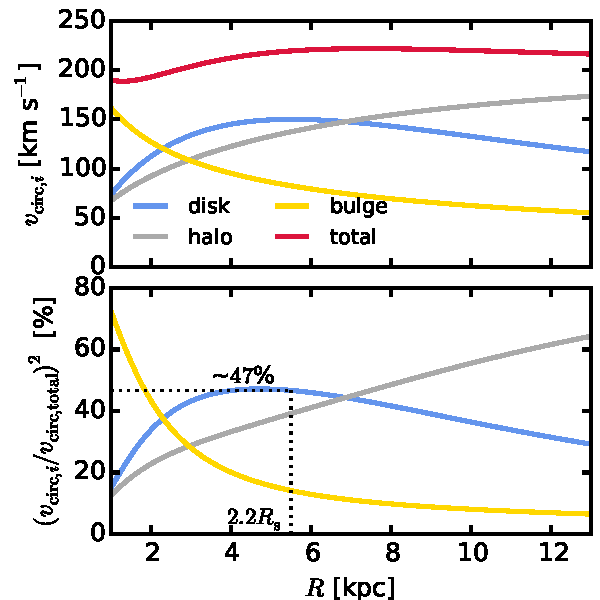
\includegraphics[width=0.7\columnwidth]{fig/plot_vcirc_decomposed.pdf}
\caption{\Answer{Circular velocity curve and fractional contribution to the radial force (rotational support) of the disk, halo and bulge components of the \texttt{DEHH-Pot}, the symmetrized best fit to the $N$-body simulation. This demonstrates that the simulation is a disk-dominated spiral galaxy.}}
\end{figure}
%====================

\paragraph{Aspect 2: Amplitude of spiral arms (continued):} The model considered here, almost axisymmetric (the contrast of the spiral structure is in its large majority less than or equal to 10\% in stellar surface density, as shown in Figure 2),  is therefore very far from the reality of the MW, and can be highly deceiving for the MW results to come. \hl{A lot of spiral structure outside of the solar radius is indeed 10\% in surface density. How to answer to this concern?}

\Answer{On "Aspect 2: Amplitude of spiral arms": The regions from which we draw our data have a very strong spiral contrast, as can be seen in Figure 2d.}

\paragraph{Aspect 4: Conservation of actions} The fact that the DF is still expressed in terms of integrals of motion, which should not be any more conserved, is a questionable issue. \hl{How to answer to this?}

\paragraph{Aspect 5: Radial migration and MAP concept:} Moreover, we know that spiral structure will trigger radial migration of stars, the
more so that there velocity dispersion is small. So for a given stellar population,
with a given metal abundance (and alpha/FE ratio), we expect that a dispersion will
occur in orbits, and the MAP concept will no longer be valid. \hl{How to answer to this?}

\paragraph{Question 1: Corotation of spiral arms} About this problem, it will be also useful to mention where is the corotation of the
spiral in the N-body model, is it near the Sun radius? \hl{How to answer to this?}

\paragraph{Aspect 5: Thick disk:} Another simplification of the N-body model is that there is no thick disk, while in
the MW, there is one which is about comparable mass to the thin disk. How will the
presence of this other components change the study of the orbits, and derivation of
the potential? \hl{How to answer to this?} 

\Answer{On "Aspect 5: Thick disk": Yes, we don't have a thick 
disk, but because by construction of the model the disk is very cold at 
2 scale -lengths our model has the maximal response of the disk to 
perturbations, and this is one of the conditions in which we wanted to 
test RoadMapping.} \hl{Not sure what Elena means.}

\paragraph{Aspect 6: No spiral arms outside of the solar radius.} Another issue is that the model considered has spiral arms only within the solar
radius, and is axisymmetric in the outer parts. Not surprisingly, there are big
departures from the true DF inside the solar radii, and less outside, as shown in
Figure 3. This will not be the case for a realistic MW model. \hl{The referee has a point that Figure 3 looks as if there were no spiral arms outside of the solar radius.}

\Answer{On "Aspect 6: No spiral arms outside of the solar radius": In the 1D spatial histograms the impression that there were no spiral arms outside of the solar radius is strengthened by averaging over the other two spatial coordinates.}

\paragraph{Aspect 2 \& 3 (continued):} p.19 in the conclusion: the authors conclude that their model has "has stronger spiral arms than we expect in the MW", which is not true, given the dominance of
the dark matter

\paragraph{Aspect 7: Number of spiral arms} It should also be recalled that in the MW when the true stellar component is mapped
in the NIR, the number of spiral arms turns out to be 2 only, while it is more 4
arms when Halpha and young stars are considered. This means that gas and star
formation are participating to harmonics and branching, but the basic stellar
structure is 2-armed. This will modify the conclusion, since the importance of
spiral arms in the stellar structure will be higher. \hl{How to answer to this?}

\paragraph{Task 1: Callibrating the method using smooth data.} There is also some issue which is striking in the paper, is that the departures from
the model are very high, when looking at Fig 3, 6 or even 11. And the reader wonders
how much is due already to the N-body model without spiral arms. Therefore it might
be interesting to calibrate the method, using the snapshot T=0 (or close to 0), the
initial axisymmetric model without spiral arms, and apply RoadMapping to understand
the  influence of the basic model. This might not be a long task, only providing a
test, or a Figure, but certainly will help to understand the high discrepancy
between derived results and the model.

\paragraph{Comment regarding the software policy:}

Per the new AAS software policy, http://journals.aas.org/policy/software.html, the
authors should use AASTeX v6.1 for the revised manuscript to highlight the code they
used with the new {\textbackslash}software command, e.g.

{\textbackslash}software{GADGET-3 (Springel et al. 2005), galpy (Bovy 2008), emcee (Foreman-Mackey
et al. 2013)}

\section{List of TO DOs for Wilma}


\begin{enumerate}
\item Mention in abstract, introduction, Section 2.5 and discussion/conclusion 
\begin{itemize}
\item ... that our model does not have a bar and that this is indeed a limitation of the methodology used in this paper. 
\item ... that ultimately we are not trying to analyze the most realistic non-axisymmetric MW simulation
\end{itemize}
\item Write new Section 2.5 that explicitly addresses how the non-axisymmetry in the N-body snapshot compares to what we know in the MW. Aspects to discuss:
\begin{enumerate}
\item no bar (but bar importance will be small outside the bar region in the MW) \hl{what?}
\item number of arms:  We have 4 arms instead of 2. Well  we don't have the gas. I think adding the gas component might help that. In any case the number of arms in our Galaxy is still very uncertain, so this is not a major point. \hl{I don't get Elena's point with the gas and spiral arms?}
\item spiral arm strength \hl{how?}
\item streaming motions are much larger than in MW (forward reference to Figure 3, compare to results of Reid et al. 2014; make sure not to mention it in Section 5.4 then; "A local spiral arm
density wave, for example, can impose kinematic fluctuations on the order of 10 km/s (Siebert et al. 2012)." from Bland-Hawthorn \& Gerhard 2016)
\item disk scale length similar to MW (2.5 kpc here vs. $2.15\pm0.14$ kpc in Bovy \& Rix 2013; $2.6\pm0.5$ kpc according to review by Bland-Hawthorn \& Gerhard 2016); 
\item disk scale height slightly smaller  (here 170 pc; 220–450 pc for thin disk according to Bland-Hawthorn \& Gerhard 2016)
\item halo fraction \hl{how?}
\item no gas disk
\item no stellar thick disk
\item co-rotation radius of spiral arms \hl{how?}
\end{enumerate}
\item Check claims of referee:
\begin{itemize}
\item Find out if the bulge mass is really 25\% of the stellar disk mass?
\item Find out how the referee came to the conclusion that the stellar disk mass fraction is only 4\%? In reality this must be closer to 50-50 (since 4\% is out to 100s of kpc)?
\end{itemize}
\item plot of the rotation curve and its decomposition into components in the DEHH model (and maybe of the simulation)
\begin{itemize}
\item ... to demonstrate that stars and DM contribute \textasciitilde equally to the rotation curve (or at least at more than 4\%!) and galaxy is NOT dark matter dominated in the inner parts. 
\item ... show that indeed the disk fraction at 2 scale-lengths of the disk is 50\%. (This is enough to generate low number of arms and with high strengths.)
\end{itemize}
\item Plotting the strength of the spiral arms
\begin{itemize}
\item Elena suggests: You can show the strengths of arms computing the dominant modes as a 
function of the radius (m=2,m=4 maybe m=5 or m=6). The amplitude of the 
fourier mode analysis will show also the strengths of the arms (although 
the mode analysis is quite noisy but it is worth to give a try). m=2 and 
4 will dominate within the solar radius but higher m are also present in 
the outer parts. \hl{How to do that?}
\end{itemize}
\item Visualizing images with a larger contrast. 
\begin{itemize} 
\item Elena suggests: Can you use a color bar 
where the constrast is enhanced? It will show the complex spiral 
structure present in the simulation. For example the referee comments 
that the model has spiral arms only within the solar radius. This is not 
true, as you can see in D'Onghia 2015 (the top left panel in Fig.2) 
there are other weaker arms even outside the solar radius (2 scale 
lengths) but your image doesn't show them. \hl{I'm not a big fan of using a "stripey"-looking colormap in my Figures 1 and 2...}
\item Another way to show the 
strengths of the spiral structure and how they perturb the potential is 
to show the gravitational potential at t=250 Myrs as in Fig.6 (bottom 
panel) of Vera-Ciro, D'Onghia et al. 2014. \hl{Just for the particle potential stored as POT keyword with the simulation keyword? Or also the halo potential?}
\end{itemize}
\item Run analysis for snapshot snap\_000.hdf5 to calibrate method. This could be a small appendix. \hl{What plots would be interesting to see?}
\end{enumerate}

\end{document}